To get a better overview of the error, 
we have made a graph of the error for different degrees of the polynomial 
and different sizes of $h$.
This makes it more managable to see how the the different degrees and mesh 
sizes affect the error. We start by discussing the $L_2$ error.
We see on Figure~\ref{fig:l2-fejl-plot} that in general the error 
decreases as the degree of the polynomial increases and as the size of 
$h$ decreases, so does the norm, 
although this is not the case for all mesh sizes.
We see that the error decreases as the mesh size decreases up 
to polynomials of degree $8$, 
which can be seen more accurately in Table~\ref{tab:convergence_l2}, 
but this changes for polynomials of degree $8$, $9$, and $10$.
This should not be the case, 
but could be due to the size of the error, which is so small the 
rounding errors could become more significant.
The $H^1$ error shown on Figure~\ref{fig:h1-fejl-plot} generally 
has the same tendency as the $L_2$ error, 
but as mentioned earlier the error is generally higher.
However, the order of polynomial, where the tendency changes is 
different for the $H^1$ error, as it changes at degree $9$ instead of $8$, 
see Table~\ref{tab:convergence_H1}.
Furthermore, after the change in tendency, 
the error does not increase as drastically as for the $L_2$ error. 

\begin{figure}
    \begin{centering}
    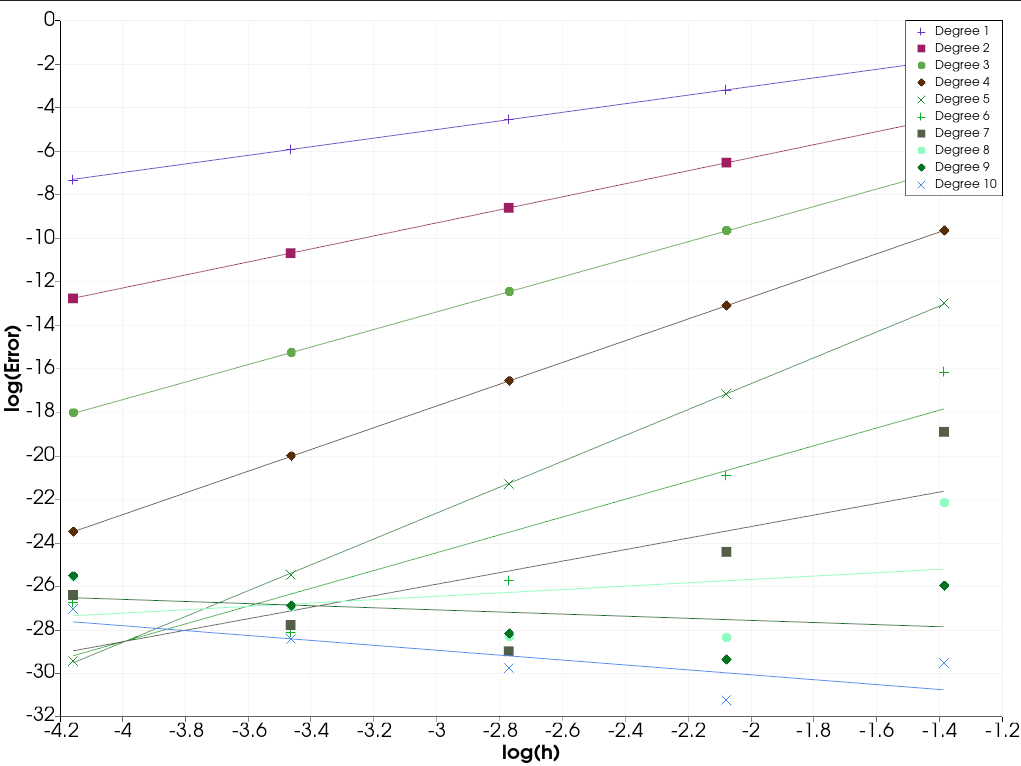
\includegraphics[width=0.8\textwidth]{Afsnit/Application/figurer/l2-fejl-plot.jpeg}
    \caption{Plot of the $L_2$ error for the different degrees of the polynomial and different sizes of $h$.}
    \label{fig:l2-fejl-plot}
    \end{centering}
\end{figure}

\begin{figure}
    \begin{centering}
    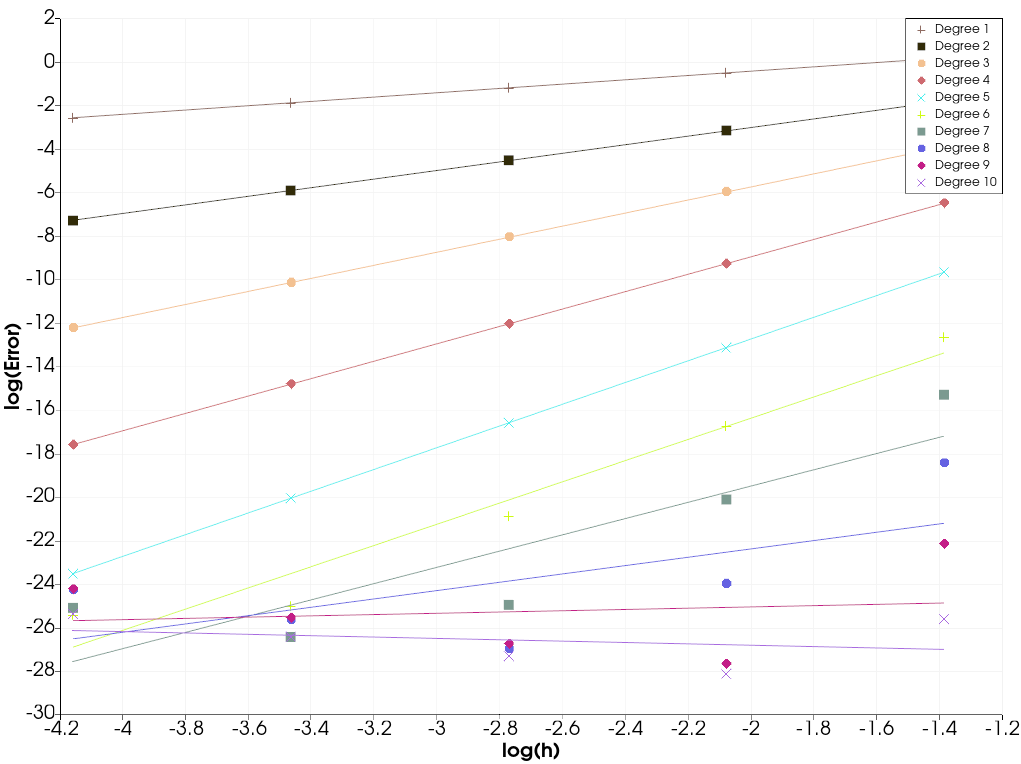
\includegraphics[width=0.8\textwidth]{Afsnit/Application/figurer/h1-fejl_plot.png}
    \caption{Plot of the $H^1$ error for the different degrees of the polynomial and different sizes of $h$.}
    \label{fig:h1-fejl-plot}
    \end{centering}
\end{figure}

In general the numerical experimentation agrees with the theory, though 
for high degree of polynomials we get conflicting information. We are unsure 
as to the exact reason, as changing the way the errors are calculated, both 
using the $H^1$-norm and $L_2$ norm, and increasing the degree used to calculate 
errors in the practical function did not change this outcome.